\documentclass[12pt,a4paper]{report}
\usepackage{graphicx}
\usepackage[turkish]{babel}
\usepackage[utf8]{inputenc}
\usepackage{hyperref}

\begin{document}
	\begin{titlepage}
		\centering
		\shorthandoff{=}
		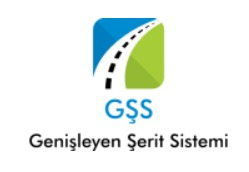
\includegraphics[width=0.5\textwidth]{logo.jpeg}\par\vspace{1cm}
		{\scshape\LARGE Gebze Teknik Üniversitesi \par}
		\vspace{1cm}
		{\scshape\Large BIL101\par}
		\vspace{1.5cm}
		{\huge\bfseries Proje Raporu\par}
		\vspace{2cm}
		{\Large\itshape Grup 4\par}
		\vfill
		Nurettin Cem \textsc{Dedetaş}\par
		Yiğit Yağız \textsc{Çaktı}\par
		Ömer Faruk \textsc{Bitikçioğlu}\par
		Gökçe Nur \textsc{Erer}\par
		Haktan Bilgehan \textsc{Dilber}\par
		Mevlüt Reha \textsc{İnan}\par
		Jerfi İlkcan \textsc{Ceylan}
		\vfill
	
		{\large 8 Aralık 2017\par}
	\end{titlepage}

{\Large\bfseries Problem Tanımı \\ \par}

Herkesin sıkça karşılaştığı , trafikteki araçların tek bir yöne ağırlık vermesi ; bu sebepten dolayı yolların etkin kullanılamaması ve yolların büyük bır kısmı boşken trafik sıkışıklığının meydana gelmesi sorunu ele alındı. \\ \\

{\Large\bfseries Amaç \\ \par} 
Amaç , o anda aktif olarak kullanılamayan şeritlerin ; yolların olabilecek en yüksek verimde kullanılması için trafik yoğunluğuna bağlı olarak karşılıklı yönler arasında dağıtlımasını sağlamak. \\ \\

{\Large\bfseries Çözümümüzün Kısa Özeti \\ \par} 
 Problemde de belirttiğimiz gibi, yol yönlerinin birinin yoğunluğu çok fazla iken öteki yönün yoğunluğunun az olduğu durumlarla çok karşılaşıyoruz. Sistemimiz yoğunluğu az olan yöndeki şeridi yoğun olan bölgeye vermek için çalışacaktır. Öncelikle sistemimiz trafiğin yoğun olduğu bölgeleri belirleyecek. Sonra bu yönde şerit açabilmek için karşı yönün trafik yoğunluğunu kontrol edecektir. Eğer şerit sayısının azalması yoğunluğu yüksek derecede arttırmayacaksa, az yoğun olan bölgeden bir şeridi karşı yöne doğru açacaktır. Bütün bunlar için ise araçların uygun şeritlere yönlendirilmesi, otonom arabalarda; gitmeleri gereken şeridin araçlara bildirilmesi, otonom olmayan arabalarda ise sürücünün uyarılması gerekmektedir.\\
 
 Genişleyen Şerit Sistemi ana otoyollarda kullanılmak için tasarlanmıştır. Köprü veya az şeritli dar yollarda kullanılmamaktadır.\\
 
 Otonom olan araçların yazılımlarına dahil edilecek kontrol sistemi, otonom olmayan arabalarda ise ayrı bir gömülü sistem olarak eklenecektir. Bu gömülü sistemin yeni üretilen araçlarda olma zorunluluğu bulunacaktır. Eski araçların da bu gömülü sistemi yasal olarak edinmeleri gerekecektir. \\ \\ \\
 
{\Large\bfseries Sistemdeki Aktörler\par}
\begin{itemize}
	\item \textbf{Araçlar\\}
	o	Sistemin en önemli aktörü olan kullanıcı kitlesi.
	\item \textbf{Kameralar\\}
	o	Trafiğin devamlı görsel verilerini toplayıp işlemesi için sunuculara sağlar.
	\item \textbf{Sensörler\\}\
	o	Sistemin devamlı doğru çalışması için sürekli bir kontrol mekanizması oluşturur.
	\item \textbf{Sunucular\\}
	o	Kameralar ve sensörlerden gelen veri yığınından gerekli verileri ayırır ve sistemi çalıştırır / yönetir.
\end{itemize}
\shorthandoff{=}
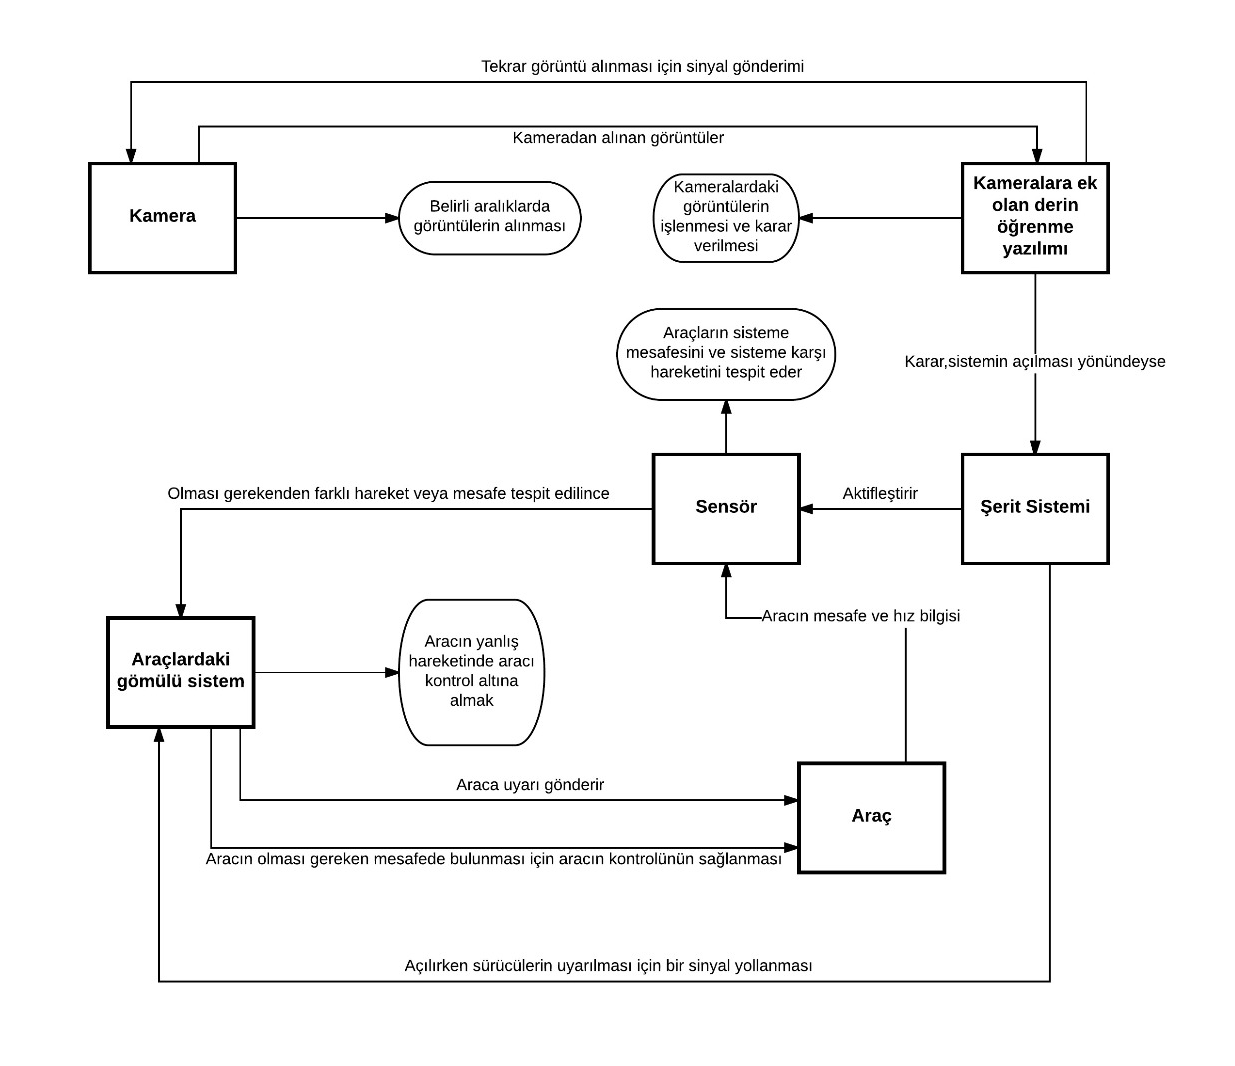
\includegraphics [width=\linewidth]{usecase.png}
\shorthandoff{=}
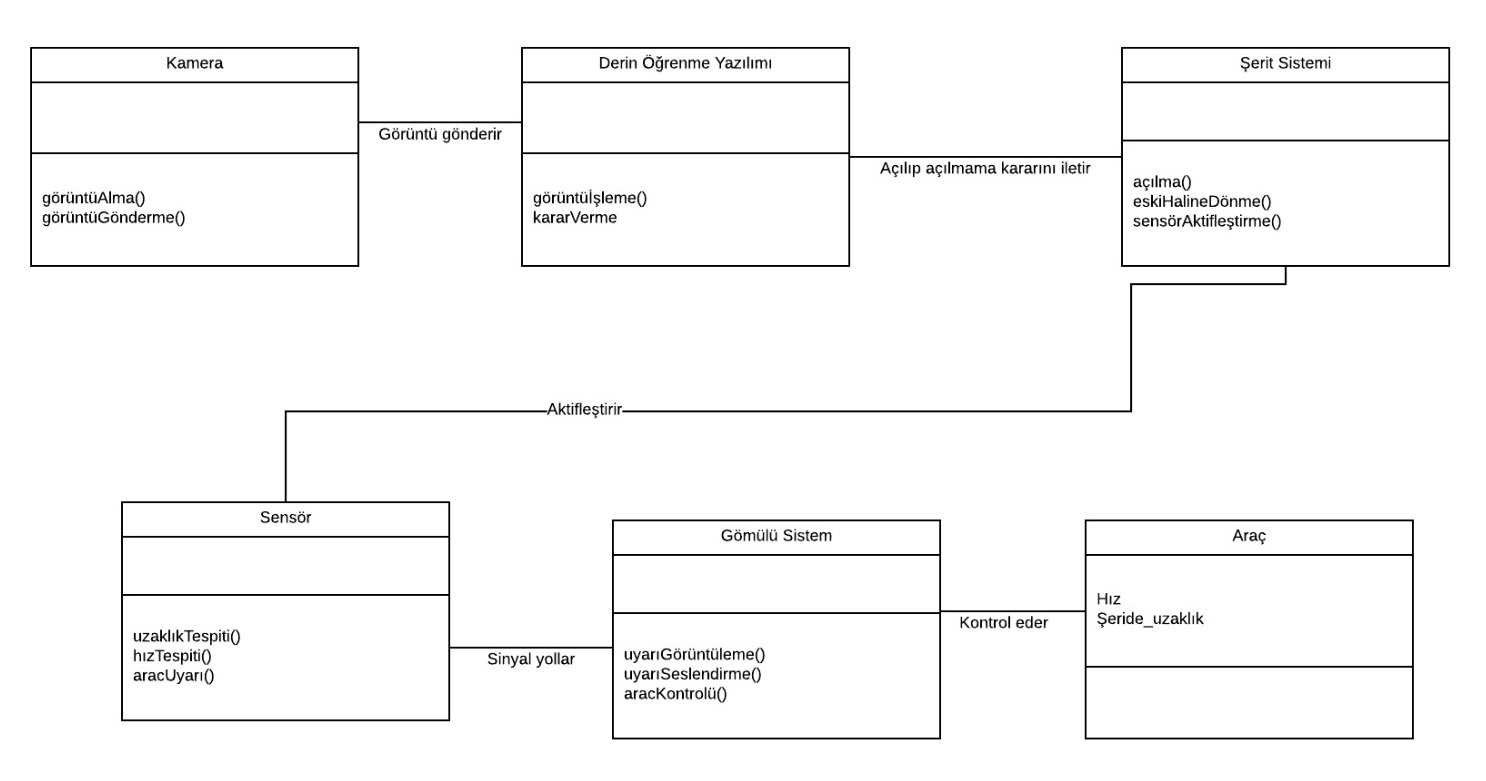
\includegraphics [width=\linewidth]{uml1.jpg}
\shorthandoff{=}
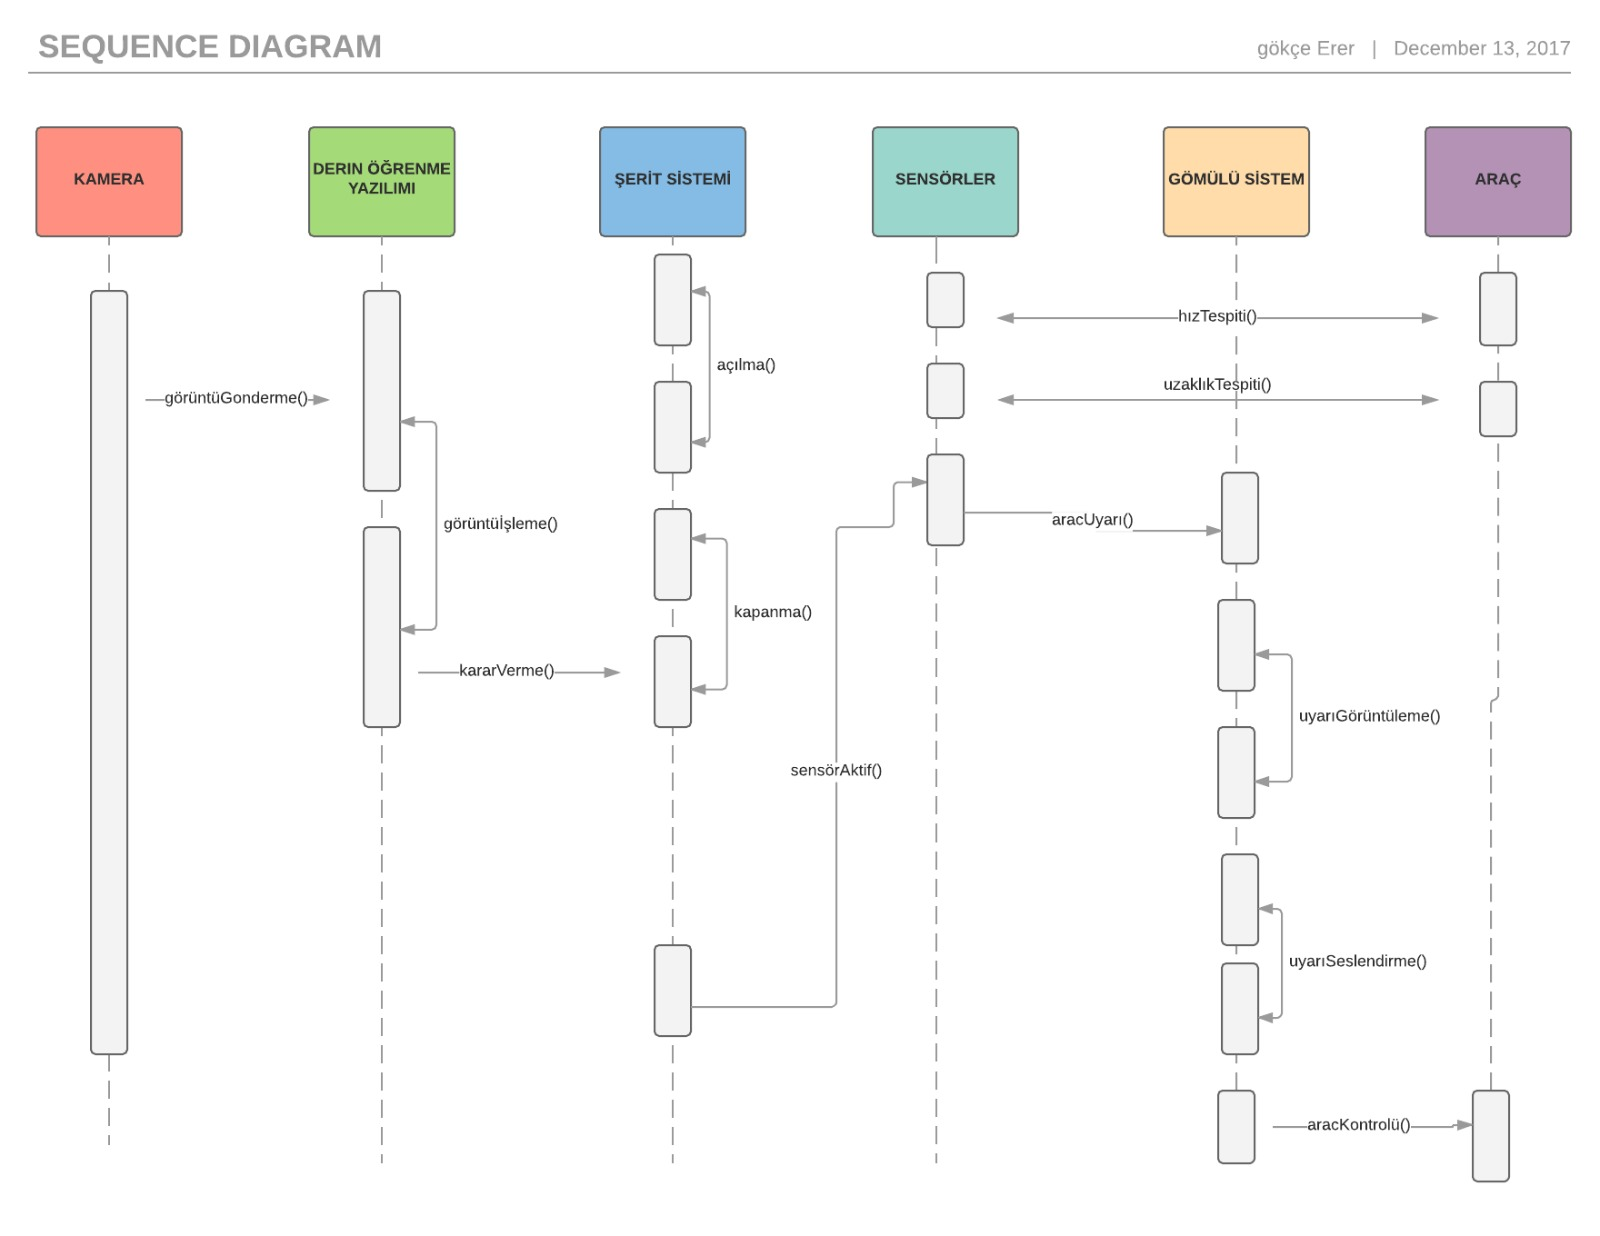
\includegraphics [width=\linewidth]{uml2.jpg}
\newpage
{\large\bfseries Kullanılan Teknolojiler ve Projedeki Kullanım Alanları\\ \par}

{\normalsize\bfseries Veri Madenciliği \\ \\}
Veri Madenciliği ,son 10-20 yılda hem verin saklanması hem de veriyi işleyecek bilgisayarların güçleri artarken bir yandan ucuzlaması sebebiyle hızla gelişmekte olan bir teknolojidir.Bu teknolojinin temelinde yığın halindeki verilerden , belki o verilerin yüzde 1’ini bile oluşturmayan fakat gerekli / kullanışlı olan bilgileri ayıklamak yatmaktadır. \\

Bu projede veri madenciliğinin kullanım alanı ise kamera ve sensörlerden gelen verileri , derin öğrenme algoritmasında kullanılması için fazlalıklarından ayırıp işlenebilir hale getirmektir. \\ \\

{\normalsize\bfseries Derin Öğrenme \\}

Derin öğrenme GPU yardımı ile girdi olarak alınan bilgileri sınıflandırarak ilerleyen bir makina öğrenmesi dalıdır.\\

Bu projede otonom araçlarda hangi durumların optimal olduğunu ve aynı zamanda şerit değiştirme gereksinimde nasıl bir hareket izlemesi gerektiğine karar verilmesi için kullanılmaktadır.\\

Otonom olmayan araçlarda ise aracın içine eklenmiş bir gömülü sistem yardımı ile alinan bilgilerden hangi durumda aracın kontrolünün şöförden alınması gerektiğine ve kontrolün alınması durumunda ne yapılacağına karar vermektedir. \\ \\

{\normalsize\bfseries Gömülü Sistemler \\}

Gömülü sistem, bir sisteme akıllılık özelliği katan yazılım ve donanım bütünüdür. Gömülü sistemler içinde kullanılan yazılımlar normalde bilgisayarda kullandığımız programlara göre daha özel amaçlarla oluşturulmuştur. Yani belirli bir fonksiyonu gerçekleştirmek için tasarlanmışlardır. Gömülü sistemler genel olarak bellek ve mikrodenetleyici kısımlarından oluşur. Girdiler mikrodenetleyicilere belirli donanımlardan (klavye,sensör vb.) girip, çıktılar da yine mikrodenetleyiciden gerekli donanım parçasına (lcd ekran, gösterge vb.) iletilmektedir. \\

Gömülü sistemler güvenilir olmalıdır ve bir hata durumunda, hatası tolare edilebilmelidir. Çünkü projemizde de olduğu gibi gömülü sistemler hayatımızı tehlikeye sokabilecek durumları engellemek için de kullanılmaktadır. \\

Gömülü sistemlerin projemizde kullanım amaçlarından biri sensörlerden gelen bilgilere göre şerit sisteminin hareketini sürücüye bildiren uyarıyı oluşturmaktır. Gömülü sisteme sensörlerden gelen bilgi mikrodenetleyicisinden geçerek gösterilmesi gereken görüntülü uyarıyı aracın içindeki ekrana bastırır. Gömülü sistemlerin projemizde kullanıldığı başka bir amaç ise aracın şerit sistemine karş yaptığı ters bir harekette aracın kontrolünün sağlanması. Yine sensörlerden gelen bilgiler araçta bulunan gömülü sisteme iletilerek aracın direksiyonunun kontrolünün sağlanması için gerekli donanım parçalarına gerekli sinyalleri gönderir. \\ \\

{\normalsize\bfseries Görüntü İşleme \\}

Görüntü işleme, verilen görüntülerden yararlı bilgiler çıkarmak üzerine yoğunlaşmış bir bilgisayar bilimleri teknolojisidir. Burada verilen görüntü bir resim, fotoğraf veya bir video kesiti olabilir. Görüntü işlemenin aşamaları arasında görselleştirme, görüntü keskinleştirme ve restorasyon, görüntü alımı, desen tanıma ve görüntü tanıma yer alır. \\ \\

Görüntü işleme teknolojisinin projede kullanılmasının sebebi yollarda bulunan kameralardan alınan fotoğrafların işlenerek fotoğraflarda bulunan araçların yoğunluğunun tespit edilmesidir. Bunun gerçekleştirilmesi için trafik kameralarıyla alınan görüntü ilk önce çevresel nesnelerden arındırılır. Bu nesnelere yol ve kaldırımlar örnek olarak gösterilebilir. Bu aşamadan sonra resimdeki öğelerin gri tonlaması yapılır. Bu yapılırken teker teker piksellerin kırmızı-yeşil-mavi değerleri siyah değerine çevrilir. Bu işlem kenarların tespit edilmesini kolaylaştırır. İşlemin son aşaması olan kenar tanımlama sayesinde arabaların tespiti sağlanır ve veriler sisteme aktarılır. \\ \\

\newpage

{\large\bfseries Detaylı Tasarım Açıklaması\\ \par}

Genişleyen şerit sisteminin çalışma sistemi şu şekildedir: \\

Kameralar: Kameralardan trafiğin durumuna ait belirli zaman aralıklarıyla görüntüler alınır. \\

Derin Öğrenme Yazılımı:  Kameralara ek olan derin öğrenme yazılımı gerekli alınan görüntüleri işleyerek çeşitli sonuçlar çıkarır. Bu sonuçlar arasında sistemin açılıp açılmayacağına karar vermede etkili olacak sonuçlar, veri madenciliği algoritmalarıyla ayrılarak karar verilir. \\

Sensörler: Derin öğrenme yazılımının verdiği karara göre sensörlere uyarı gönderilir ve sensörler araçlara sistemin hareketine dair bir uyarı gönderir. Ardından sensörler araçların hareketine dair bilgi toplamaya başlar. Araçların kazaya sebebiyet verebilecek hareketlerinde sensörler araçların gömülü sistemlerine gerekli sinyali yollar. \\

Araçların gömülü sistemleri: Sensörlerden gelen sinyallere göre araçtaki gömülü sistemin ekranında sürücüyü/yolcuyu uyaran uyarıların gösterilmesini sağlar. Ayrıca aracın kazaya sebebiyet verebileceği durumda ise gömülü sistem aracın direksiyon kontrolünü ve fren kontrolünü ele geçirerek aracın kontrolünü sağlar. \\ \\

\newpage

{\large\bfseries Sistemin Avantajları ve Dezavantajları\\ \par}

{\normalsize\bfseries Avantajlar: \par}

\paragraph{Yolların kullanılımı optimize eder:} Yollarda sistem kullanılmadığında boş kalacak yerleri kullanıma açar. \\

\paragraph{Trafik yoğunluğunu azaltır:} Trafik ter bir tarafa ağırlık vermesindense iki yöne eşit dağılır ve yoğunluk azalır. \\

\paragraph{Zamandan tasarruf sağlar:} Tek bir tarafın hızlı gitmesindense iki tarafta da boş yol miktarı eşitlenerek hız dengesi sağlanır. \\

\paragraph{Yakıt giderlerini azaltır:} Durup kalkarken duruş sırasında boşa harcanan yakıt miktarını azaltır , ortadan kaldırır. \\

{\normalsize\bfseries Dezavantajlar: \par}

\paragraph{Güncel teknolojilerin yetersizliği:} An itibari ile otonom araçların yollara açık olmaması ve kullandığımız gömülü sistem teknolojisinin ulaşılabilir olmaması. \\

\paragraph{Yüksek maliyet:} Tüm araçların otonom olması ya da bu gömülü sistemin eklenmesi maliyetlerinin yanında yolların rahat değişmesi için ortadaki bariyerlerin kaldırılması maliyetli bir işlemdir.

\newpage
{\large\bfseries Çözümün Geliştirilebilir Yanları: \par}

\begin{itemize}
	\item Şerit sisteminin kaza oluşturma riski daha da azaltılabilir.
	
	\item Araçların kontrol sistemi geliştirilebilir.
	
	\item Şerit sisteminin kurulma maliyeti azaltılabilir.
	
	\item Sistem bozulduğunda şeritleri düzenleyecek bir arka plan çözümü geliştirilebilir.
	
	\item Sistemin köprülerde kullanılması sağlanabilir.
\end{itemize}

{\large\bfseries Kullanıcı Senaryoları: \par}

\begin{itemize}
	\item Şerit sistemi açılırken araç şerit sistemine ters bir yönde/harekette ise;
	
	Sensör aracın içerisinde bulunan gömülü sisteme sinyal gönderip, sürücüye gerekli uyarının verilmesini sağlar. Eğer sürücü/araç aracın kontrolünü sağlamazsa gömülü sistem sürücü/araç yerine bu kontrolü sağlar.
	
	\item Şerit sistemi açıkken araç şerit sistemine uygun bir harekette ise;
	
	Sensörlerden veri toplanmaya devam eder. Anormal bir hareket görülmediği sürece bu devam eder.
\end{itemize}

{\large\bfseries Sistemin Riskleri: \par}

\begin{itemize}
	\item Sistemimiz trafikte hareketli olacak bir sistem olduğundan dolayı araçların ani hareketlerine karşı bir çözüm yöntemimiz olmasına rağmen riski 0’a indirmemiştir. Sabit duran bariyerlere göre kaza riskini arttırmaya eğilimi vardır.
	
	\item Bariyer sistemi kontrolünü kaybederse araçlara zarar verebilecek durumlar oluşturabilir.
\end{itemize}

\newpage
{\large\bfseries Geliştirme Süreci\\ \par}
\begin{itemize}
	\item 10 Kasım- Toplantı: Probleme karar verildi. Potansiyel çözümlere karar verildi. 
	
	\item 14 Kasım- Toplantı: Proje önerisi yazıldı.
	
	\item 17 Kasım- Toplantı: Potansiyel çözümlerden optimal olanı seçildi. Teknolojiler hakkında konuşuldu. 
	
	\item 27 Kasım- Toplantı: Gönderilmiş olan proje önerisi hakkındaki geri bildirimler üzerine yeni çözümler getirildi.
	
	\item 28 Kasım- Toplantı: Potansiyel teknolojiler araştırılmak üzere bölüşüldü.
	
	\item 3 Aralık- Toplantı: Bölüşülen teknolojiler hakkında araştırmalar yapılarak asıl kullanılacak teknolojilere karar verildi. 
	
	\item 4 Aralık- Toplantı : Grup içinde görev dağılımı yapıldı.
	
	\item 5 Aralık: Afiş hazırlandı.
	
	\item 8-9 Aralık :Video hazırlandı.
	
	\item 8-9-10 Aralık : Sunum ve rapor hazırlandı.
\end{itemize}

\newpage

{\large\bfseries Görev Dağılımı\\ \par}
\begin{itemize}
	\item Trafik konusu ile ilgili özgün bir problem bulmak ve problemin tanımlanması, teknik olarak ifade edilmesi : Cem, Gökçe, Haktan , Jerfi , Ömer, Reha, Yağız
	
	\item Konu ile ilgili literatür taraması: Cem, Gökçe, Haktan , Jerfi , Ömer, Reha, Yağız 
	
	\item Probleme özgün bir çözüm önerisi tasarlamak: Cem, Gökçe, Haktan , Jerfi , Ömer, Reha, Yağız
	
	\item Problemin özgün çözümünde kullanılacak olan bilgisayar- teknoloji çözüm yöntemlerinin belirtilmesi ve açıklanması: : Cem, Gökçe, Haktan , Jerfi , Ömer, Reha, Yağız
	
	\item Kurulan sistemin nasıl çalıştığının açıklanması: Cem, Gökçe, Haktan , Jerfi , Ömer, Reha, Yağız
	
	\item Tasarladığınız proje sonucunda elde edilecek ürüne ait girdiler ve çıktılar: \\
	•	Video: Gökçe,Jerfi,Ömer,Reha\\
	•	Sunum:Cem,Haktan,Jerfi,Reha\\
	•	Rapor: Cem, Yağız, Ömer\\
	•	Afiş: Gökçe, Yağız, Haktan\\
	
	\item Yararlanılan kaynaklar sunuda ve raporda açıkça belirtilmelidir: Cem, Gökçe, Haktan , Jerfi , Ömer, Reha, Yağız
	
	\item Projeye ait UML diyagramlarının çizilmesi: Reha, Gökçe
	
	\item Önerilen çözüme ait olumlu ve beklenen çıktıların belirtilmesi: Cem, Haktan
	
	\item  Önerilen çözüme ait riskler veya olumsuz çıktıların tahmin edilmesi ve belirtilmesi: Cem, Haktan
\end{itemize}

\newpage

{\large\bfseries Referanslar(Kaynakça) \\ \par}

\begin{itemize}
	\item {\bfseries Visual Data Mining} (Pak Chung Wong) 
	
		{\footnotesize \begin{verbatim}
		https://pdfs.semanticscholar.org/d69a/63d9155eaaf678aad9a4803eee70e633a5e7.pdf
		\end{verbatim}}
	
	\item {\bfseries Data Mining Concepts and Techniques} (Jiawei Han)
	
		{\footnotesize \begin{verbatim}
		http://liacs.leidenuniv.nl/~bakkerem2/dbdm2007/05_dbdm2007_Data%20Mining.pdf
		\end{verbatim}}
	
	\item {\bfseries Vikipedi – Veri Madenciliği}
	
		{\footnotesize \begin{verbatim}
		https://tr.wikipedia.org/wiki/Veri_madenciliği
		\end{verbatim}}
	
	\item {\bfseries Gömülü Sistemler}
	
		{\footnotesize \begin{verbatim}
		Gerçek Zamanlı Gömülü Sistem ve Yazılım Tasarımı’nda ASELSAN Yaklaşımı 
		- Evrim Kahraman/Vedat Ünal
		
		Coskuntasdemir.net/neden-gomulu-sistemler
		
		Koddemy.com/blog/gomulu-sistemler-gomulu-sistem-yazilim-muhendisi-gozunden/
		
		\end{verbatim}}
	
	\item {\bfseries Derin Öğrenme}
	
		{\footnotesize \begin{verbatim}
		Deep learning Yann LeCun1, Yoshua Bengio& Geoffrey Hinton
		http://pages.cs.wisc.edu/~dyer/cs540/handouts/deep-learning-nature2015.pdf
		
		TED Talk
		https://www.ted.com/talks/jeremy_howard_the_wonderful_and_terrifying_implications
		_of_computers_that_can_learn
		\end{verbatim}}
	
	\item {\bfseries Görüntü İşleme}
	
		{\footnotesize \begin{verbatim}
		Welch Labs Learning to See playlist
		https://www.youtube.com/watch?v=i8D90DkCLhI
		
		Wikipedia Computer Vision Makalesi
		https://en.wikipedia.org/wiki/Computer_vision
		\end{verbatim}}
	
\end{itemize}

\end{document}